\graphicspath{{05-EMR/Figures/}}

\section{Electron Muon Ranger}
\label{Sect:EMR}

The EMR was a fully-active scintillator
detector~\cite{2016JInst..11T10007} with a granularity that allowed track reconstruction.
The EMR consisted of extruded triangular scintillator bars arranged in
planes.
Each plane contained 59 bars and covered an area of 1.27\,m$^2$.
Figure~\ref{fig:EMR} shows the bar cross section and the arrangement of the
bars in a plane.
Triangular bars were chosen so that tracks moving parallel to the
detector axis could not travel along the gaps between bars. 
Successive planes were mounted perpendicularly, so
that hits in neighbouring planes defined a position.
A single ``X--Y module'' was a pair of orthogonal planes.
The scintillation light was collected using a wavelength shifting
(WLS) fibre glued inside each bar.
At each end, the WLS fibre was coupled to clear fibres that
transported the light to a PMT.
All the WLS fibres from one edge of a plane were read out using one
single-anode PMT (SAPMT) so that an integrated charge measurement could be
used to determine the energy deposited in the plane.
The signals from the fibres emerging from the other edge of the plane
were recorded individually using multi-anode PMTs (MAPMTs). 
The full detector was made up of 24 X--Y modules giving a total active 
volume of approximately~1\,m$^3$.
\begin{figure}[htb!]
  \begin{center}
    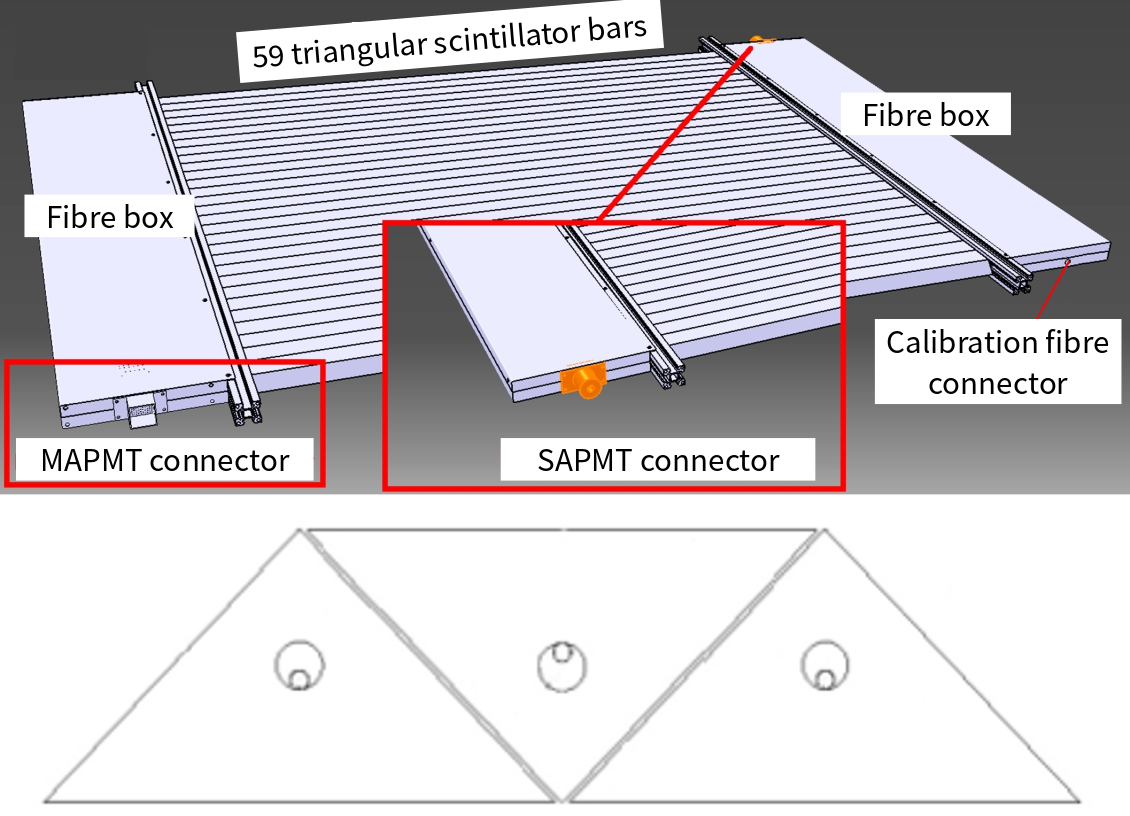
\includegraphics[width=0.465\columnwidth]{EMR1-edited.png}
    \hfill
    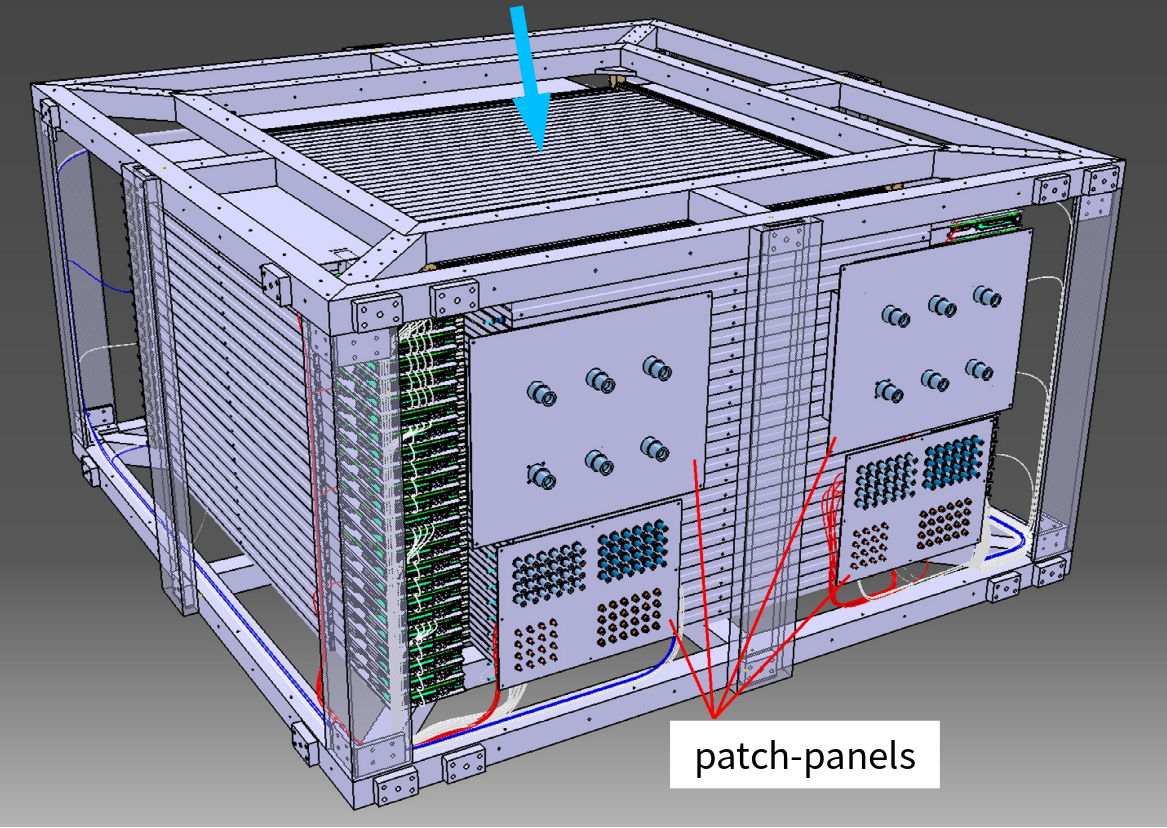
\includegraphics[width=0.515\columnwidth]{EMR2-with_beam.png}
  \end{center}
  \caption{
    Drawing of one EMR plane (top left), cross section of the
    arrangement of 3 bars and their wavelength shifting fibres (bottom
    left) and drawing of the full detector and its supporting
    structure (right).
    The beam direction is represented by the blue arrow perpendicular to the detector.
  }
  \label{fig:EMR}
\end{figure}

Measurements of the performance of the completed detector demonstrated
an efficiency per plane
of~$99.73\pm0.02$\%~\cite{2016JInst..11T10007,Drielsma:2017doj}.
The level of crosstalk was within acceptable values for the type of
MAPTM used, with an average of $0.20\pm0.03$\%
between adjacent channels and a mean amplitude
equivalent to $4.5\pm0.1$\% of the primary signal.
Only four dead bars were present.

The primary purpose of the EMR was to distinguish between a muon that crossed  the entire magnetic channel and those which decayed in flight producing an electron.
Muons and electrons exhibited distinct behaviours in the detector.
A muon produced a single straight track before either stopping or
exiting the scintillating volume.
Electrons showered in the lead of the KL and created a broad cascade
of secondary particles.
Two main geometric variables, the ``plane density" and the ``shower spread",
were used to differentiate them.
The detector was capable of identifying electrons with an efficiency
of 98.6\%, providing a purity for the MICE beam that exceeds
99.8\%.
The EMR also proved to be a powerful tool for the reconstruction of
muon momenta in the range
100--280\,MeV/$c$~\cite{2015JInst..10P2012A}.  \\

\newpage

\noindent\textbf{Performance} \\
\noindent
A full description of the detector and the reconstruction algorithms
used may be found in reference~\cite{2015JInst..10P2012A}.
Here the performance of the EMR detector over the course of the
experiment is summarised.

To measure the performance of the EMR the MICE beamline was set to
deliver a nominal momentum of 400\,MeV/$c$. This maximised the muon
transmission to the EMR and its range in the detector.
In this configuration the beamline produced pions and muons in
comparable quantities and electrons.
Time-of-flight between TOF1 and TOF2 was used to identify particle
species and only particles compatible with the muon hypothesis were
included in the analysis.
Particles entering the muon sample had a momentum larger than
350\,MeV/$c$ at the upstream surface of TOF2 and were expected to
cross both TOF2 and the KL and penetrate the EMR.
$99.62\pm0.03\%$ of the particles entering TOF2 were observed to produce
hits in the EMR.
The small inefficiency may be attributed to pions in the muon sample
that experienced hadronic interactions in the KL.
If hits were produced in the detector, an $(x,y)$ pair, defining a
space point, was reconstructed $98.56\pm0.06\%$ of the time.

To evaluate the efficiency of the scintillator planes, only the muons
that traversed the entire detector were used.
Muons were selected which produced a hit in the most downstream plane.
For these events a hit was expected in at least one bar in each plane
on its path.
The mode of the hit-multiplicity distribution per plane was one,
in $3.26\pm0.02\%$ of cases a plane traversed by a muon did not
produce a signal in the MAPMT, and the probability that the track was
not observed in the SAPMT was $1.88\pm0.01\%$. \\

\noindent\textbf{Electron rejection} \\
\noindent
A broad range of beamline momentum settings was used to characterise
the electron-rejection efficiency.
Particle species were characterised upstream of the EMR using the
time-of-flight between TOF1 and TOF2.
For each momentum setting, a fit was carried out to determine
the position of the muon and electron time-of-flight peaks and events were
selected accordingly to form muon and electron-template samples.
%For each momentum setting, a Gaussian fit was carried out to determine
%the position of the muon and electron time-of-flight peaks.
%Events which fell within {\color{red} XX standard deviations} of the
%central value of the muon time-of-flight peak were were accepted into
%a muon-template sample while events which fell within {\color{red} XX
%standard deviations} of the electron peak formed the electron-template
%sample. 
Particles with a time-of-flight larger than the upper limit of the
muon sample were either pions or slow muons and were rejected.

To distinguish the muon tracks from the electron-induced showers,
two particle-identification variables were defined based on the
distinct characteristics of the two particle species.
The first is the plane density, $\rho_p$:
\begin{equation}
  \rho_p = \frac{N_p}{Z_p+1},
\end{equation}
where $N_p$ is the number of planes hit and $Z_p$ the number of the
most downstream plane~\cite{2015JInst..10P2012A}.
A muon deposits energy in every plane it crosses until it stops,
producing a plane density close to one.
An electron shower contains photons that may produce hits deep inside
the fiducial volume without leaving a trace on their path, reducing
the plane density.
The second variable is the normalised $\hat{\chi}^2$ of the fitted
straight track given by
\begin{equation}
  \hat{\chi}^2=\frac{1}{N-4}\sum_{i=1}^{N}\frac{\text{res}_{x,i}^2+\text{res}_{y,i}^2}{\sigma_x^2+\sigma_y^2};
\end{equation}
where $N$ is the number of space points (one per bar hit),
$\text{res}_{q,i}$ the residual of the space point with respect to the
track in the $qz$ projection and $\sigma_q$ the uncertainty on the
space point in the $qz$ projection, $q=x,\,y$~\cite{Drielsma:thesis}.
This quantity represents the transverse spread of the hits produced by
the particle in the EMR.
A muon produced a single track giving
$\hat{\chi}^2$ close to one, while an electron shower produced a larger value.
The two discriminating variables can be combined to form a statistical
test on the particle hypothesis. 
Dense and narrow events will be tagged as muons while non-continuous
and wide showers will not.  
The quality of a test statistic was characterised in terms of
the fraction of the muon sample that is rejected, $\alpha$, and the fraction of the electron sample that is selected, $\beta$.

%The downstream tracker allows the reconstruction of particle momentum
%upstream of the EMR. 
%To assess the influence of momentum on contamination and loss, their
%values were calculated in 10\,MeV/$c$ momentum bins in the range
%100--300\,MeV/$c$.

The momentum of the particles was measured by the downstream tracker 
and this information used to determine the momentum dependence of the 
contamination and loss in the range 100--300\,MeV/$c$.
Figure~\ref{fig:emr_pid_mom} shows the loss, $\alpha$, and the
contamination, $\beta$, as a function of the momentum measured in
TKD.
$\alpha$ increases towards low muon momentum.
This is due both to an increase in the decay probability between TOF2
and the EMR and a decrease in the number of muons that cross the KL to
reach the EMR. 
\begin{figure}
  \begin{center}
    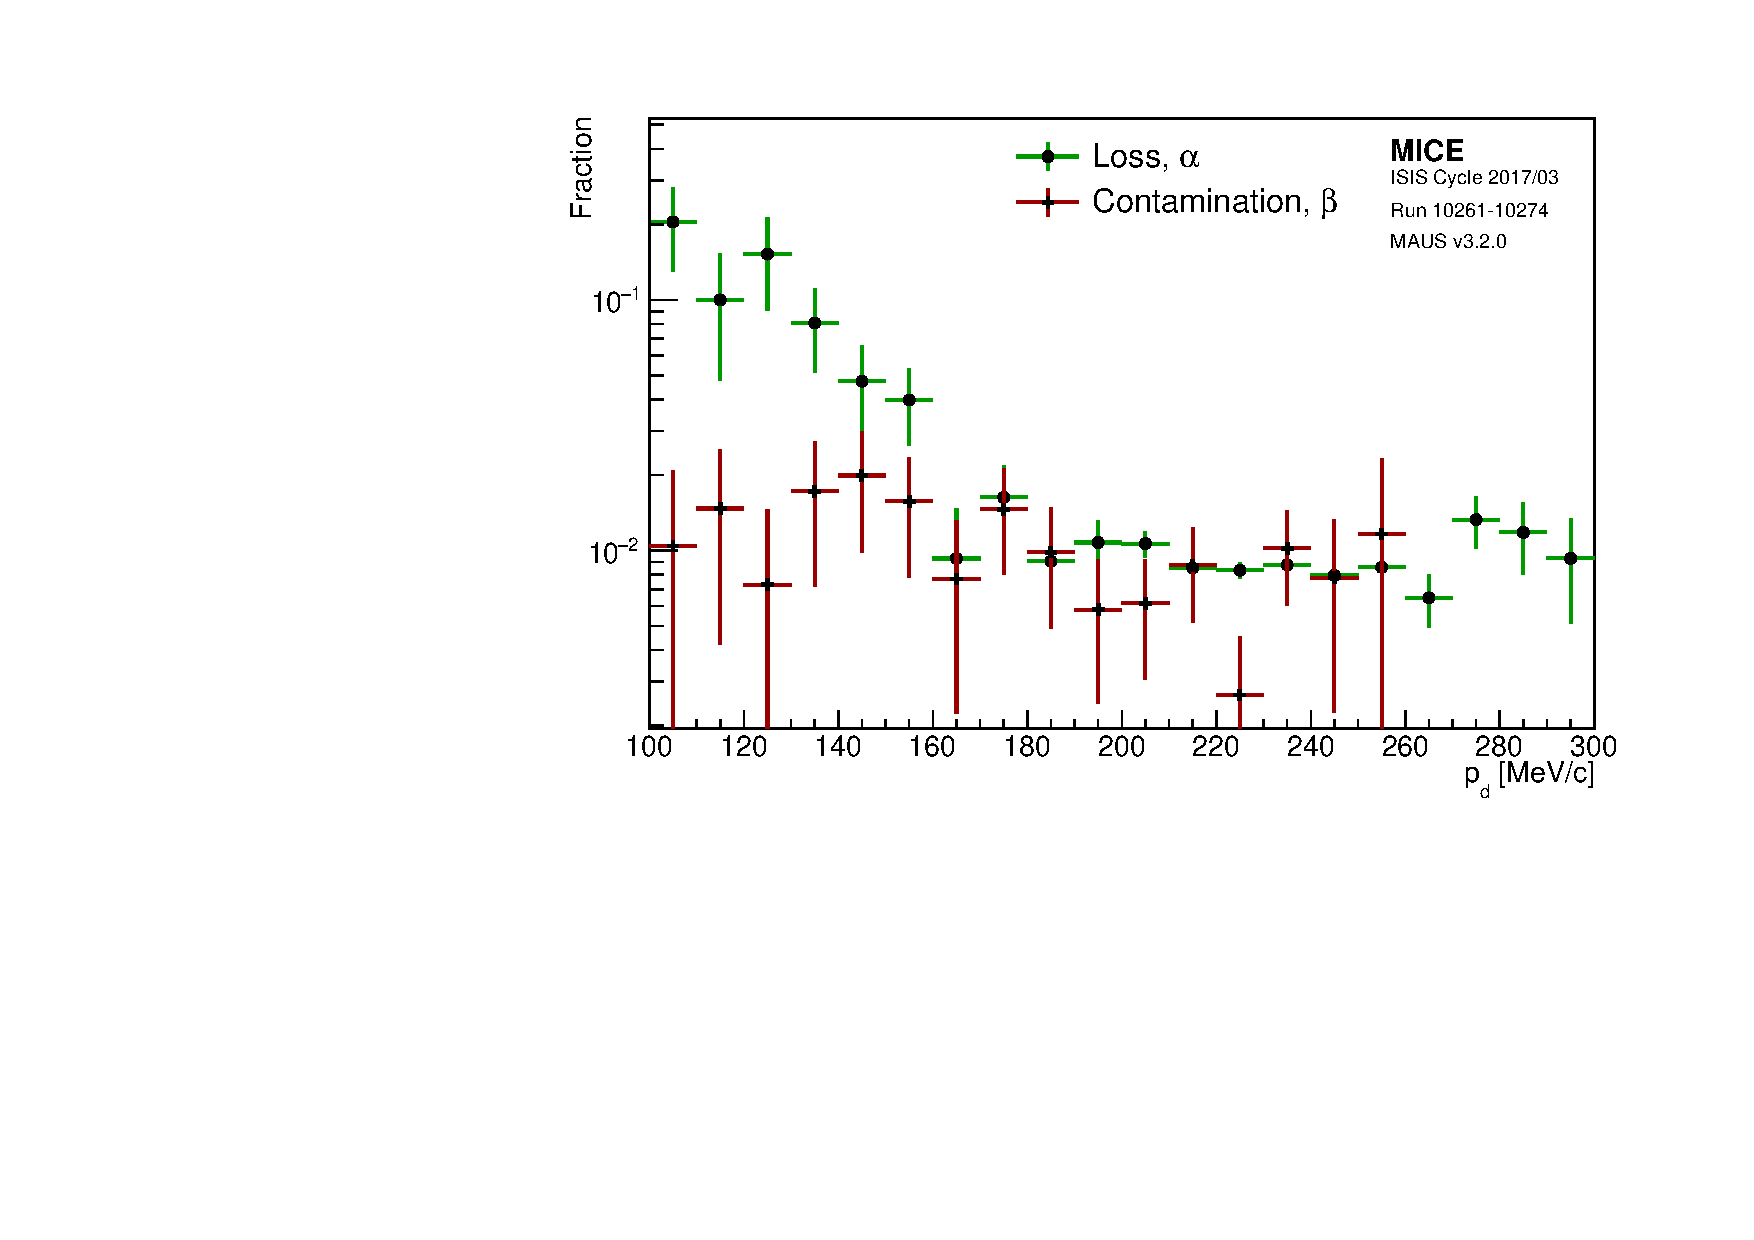
\includegraphics[width=0.68\columnwidth]{pid_mom.pdf}
  \end{center}
  \caption{
    Percentage of electron contamination, $\beta$, and muon loss,
    $\alpha$, for different ranges of momentum measured in the
    downstream tracker, $p_d$.
    The error bars are based on the statistical uncertainty in a bin,
    and the bin width set by the resolution of the measurement.
  }
  \label{fig:emr_pid_mom}
\end{figure}
